\documentclass[a4paper,fleqn]{cas-dc}
\usepackage[numbers]{natbib}
\usepackage[utf8]{inputenc}
\usepackage{graphicx}
\usepackage{xcolor}
\usepackage{array}
\usepackage{siunitx}

\usepackage{amsmath,amssymb}
\usepackage{physics}
\AtBeginDocument{\let\qty\SI}
\RequirePackage{booktabs}
\RequirePackage{textpos}
\usepackage[version=3]{mhchem}
\usepackage{float}
\usepackage{soul}

\newcommand*\mycommand[1]{\texttt{\emph{#1}}}

\begin{document}
\let\WriteBookmarks\relax
\def\floatpagepagefraction{1}
\def\textpagefraction{.001}

\shorttitle{Selective HER Activation of Monolayer CrCl$_3$}
\shortauthors{J.R. Gomez Quispe et al.}

\title[mode=title]{Selective HER Activation of Monolayer \texorpdfstring{CrCl$_3$}{CrCl3} by Transition-Metal Functionalization}


\author[1]{Juan Rafael Gomez Quispe}
\author[2]{Carlos Raul Primo Sapillado}
\author[1]{Caique C. Oliveira}
\author[2]{Chachi Rojas-Ayala}
\author[1]{Pedro Alves da Silva Autreto}\cormark[1]\ead{pedro.autreto@ufabc.edu.br}

\cortext[cor1]{Corresponding author}

\affiliation[1]{organization={Center of Natural and Human Sciences, Federal University of ABC},
    city={Santo Andre},
    state={Sao Paulo},
    country={Brazil}}

\affiliation[2]{organization={Facultad de Ciencias Físicas, Universidad Nacional Mayor de San Marcos},
    postcode={15081},
    city={Lima},
    country={Peru}}

\begin{abstract}
    Spin-polarized density functional theory calculations were performed to investigate the effect of Co, Fe, and Ni incorporation on the hydrogen evolution reaction (HER) activity of monolayer CrCl$_3$, considering both adsorbed and embedded motifs at the hollow site. The intrinsic HER activity of pristine CrCl$_3$ is first evaluated as a baseline reference, showing that its stable 2D framework requires structural and electronic activation to improve the H-binding thermodynamics. Co, Fe, and Ni bind strongly to the CrCl$_3$ surface and induce substantial structural and electronic reconstruction, including the appearance of transition-metal-derived states near the Fermi level. Among the three metals, Ni exhibits the strongest interaction with the substrate and the most pronounced perturbation of the host electronic structure, together with a tendency toward deeper incorporation during \textit{ab initio} molecular dynamics simulations. However, the strongest metal-substrate coupling does not yield the best HER response. The Co-adsorbed configuration gives the lowest H adsorption free energy, whereas Fe provides only moderate improvement and Ni remains less active.
    In contrast, the embedded configurations exhibit less active H-binding thermodynamics, suggesting that surface-exposed transition-metal sites are crucial for enhancing the HER activity.
    These results identify adsorbed Co on monolayer CrCl$_3$ as the most promising motif for HER and show that catalytic activity is governed by the interplay between local coordination, electronic activation, and H-binding thermodynamics.
\end{abstract}

\begin{graphicalabstract}
    \begin{center}
        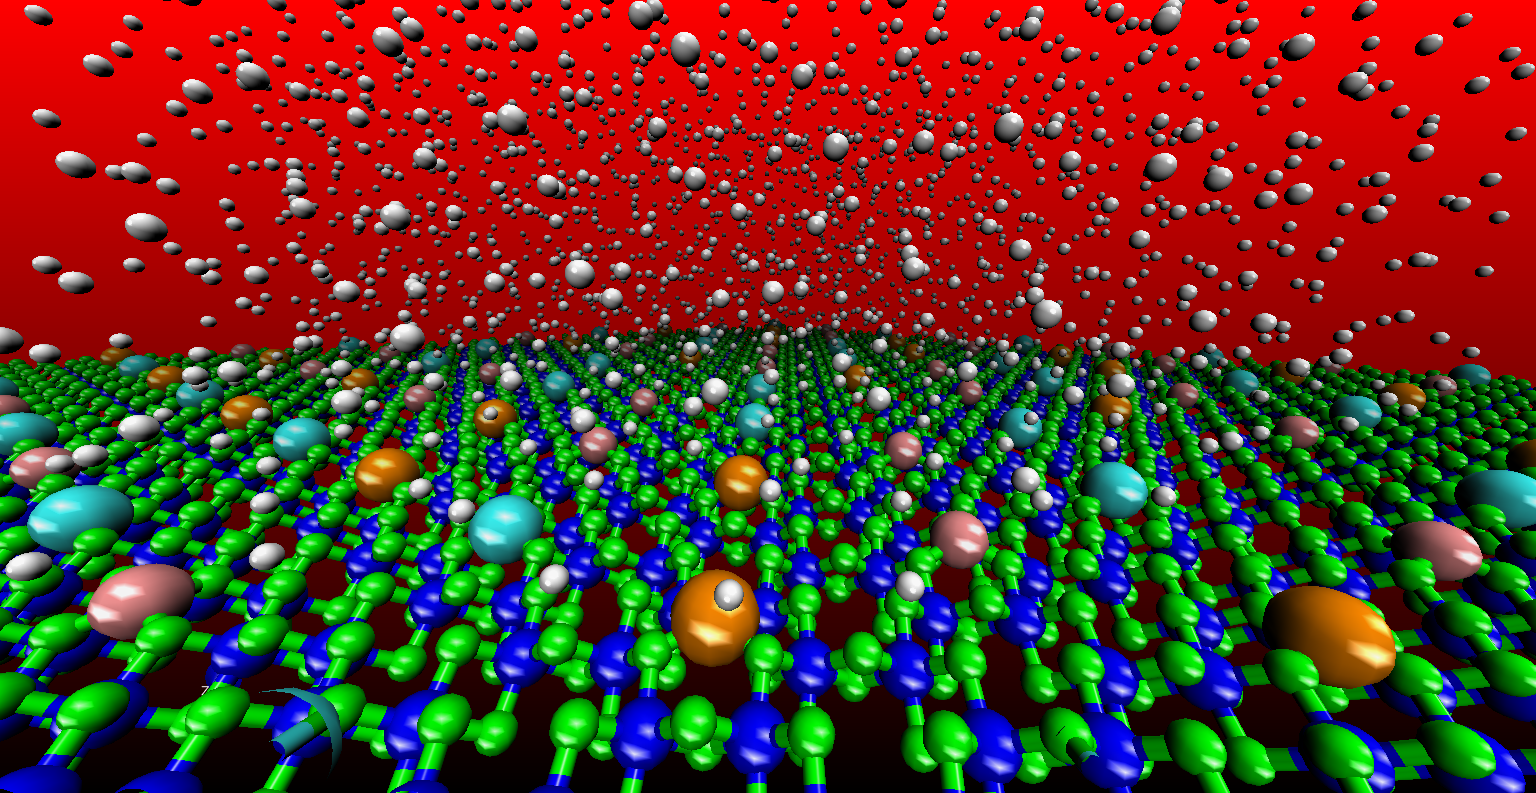
\includegraphics{figure/toc.png}
    \end{center}
\end{graphicalabstract}

\begin{keywords}
    \texorpdfstring{doped-CrCl$_3$}{CrCl3} \sep
    Hydrogen Evolution Reaction \sep
    Density Functional Theory \sep
    Ab-initio Molecular Dynamics \sep
\end{keywords}

\maketitle

\section{Introduction}

The development of efficient, stable, and low-cost electrocatalysts for the hydrogen evolution reaction (HER) remains a central challenge for sustainable hydrogen production \cite{Liao2022,Ipaves2025}. In this context, two-dimensional (2D) materials have attracted considerable attention because their reduced dimensionality, high surface to volume ratio, and chemically accessible active sites make them promising platforms for catalytic applications. Beyond conventional nonmagnetic 2D systems, intrinsic 2D magnetic materials provide an additional degree of freedom for catalyst design,
since their spin-polarized electronic structure can strongly influence charge transfer, orbital hybridization, adsorption energetics, and surface reactivity \cite{Ipaves2025}.
Among these materials, chromium trihalides (CrX$_3$, where X=I, Br, Cl) have emerged as a particularly versatile family owing to their rich interplay between electronic structure, magnetism, anisotropy, and external tunability \cite{Soriano2020,Besbes2019,Lee2026,Kvashnin2020,GarridoAldea2025}.

Within this family, monolayer CrCl$_3$ is an especially appealing platform. It is an intrinsic 2D magnetic semiconductor whose magnetic properties are highly sensitive to \textcolor{red}{spin-orbit} coupling, strain, defects, and interfacial perturbations \cite{Xue2019,Webster2018,Dupont2021,Lee2026,Zhu2025}. Importantly, CrCl$_3$ is not only a compelling theoretical platform but also an experimentally accessible material. Bulk CrCl$_3$ crystals have been successfully synthesized by chemical vapor transport \cite{Abdel-Hafiez2025} and self-transport methods \cite{Mastrippolito2021}, and atomically thin layers can be readily isolated from these crystals by mechanical exfoliation \cite{Kazim_2020}. Experimental studies have further shown that exfoliated CrCl$_3$ exhibits comparatively good environmental stability, avoiding the rapid degradation commonly observed in more reactive chromium trihalides such as CrI$_3$ \cite{Mastrippolito2021}. In addition, the fabrication of CrCl$_3$ thin layers by epitaxial and vapor-phase growth routes has also been demonstrated \cite{Bedoya2021,Wang2022}. These advances establish monolayer CrCl$_3$ as a realistic host material for exploring chemically functionalized two-dimensional magnetic catalysts.

Previous theoretical and computational studies have shown that CrCl$_3$ exhibits a comparatively weak magnetic anisotropy among chromium trihalides, which makes its magnetic state highly tunable under external stimuli such as strain, electric field, adsorption, and chemical modification \cite{Webster2018,Ebrahimian2023,Esteras2023}. In addition, its magnetism and low-dimensional character have motivated extensive investigations on exchange interactions, magnetic excitations, spin textures, and defect-driven phenomena, confirming that CrCl$_3$ is a flexible host material whose electronic and magnetic properties can be significantly reshaped by local structural or chemical changes \cite{Sarkar2021,Stagraczynski2024,Esquembre-Kucukalic2025,Lu2020,Mastrippolito2021}.

From the catalytic point of view, pristine CrCl$_3$ typically exhibits moderate HER activity, with a hydrogen adsorption free energy that requires further refinement to reach thermo-neutral binding \cite{Zala2024}. This suggests that, while the pristine material is catalytically active, its surface can be further tuned to optimize its performance for HER electrocatalysis. Therefore, chemical functionalization emerges as a promising strategy to improve its catalytic response while simultaneously exploiting its magnetic 2D nature.

Beyond its experimental accessibility, CrCl$_3$ has also been shown to be highly responsive to chemical and structural perturbations. Experimental studies have demonstrated that foreign species, defects, and related chemical modifications can substantially alter its magnetic and electronic behavior, highlighting the sensitivity of the CrCl$_3$ surface to local bonding and charge redistribution \cite{Luo2020,Gao2018,Mastrippolito2021,Mastrippolito2022}. Complementary studies on transition-metal incorporation and related modifications, such as Ni doping and Fe-doped CrCl$_3$ under pressure, further indicate that chemical modification can strongly affect the band structure, magnetic ordering, and overall stability of the system \cite{Wang2019,Abdel-Hafiez2025,Safi2023}. Taken together, these results support transition-metal functionalization of CrCl$_3$ as a physically motivated and experimentally plausible route to tailor its surface chemistry and catalytic response, even though the specific Co-, Fe-, and Ni-decorated hollow-site motifs considered here remain to be directly realized and characterized.

Nevertheless, despite the growing body of work on the magnetism of CrCl$_3$, strain effects, defects, and selected dopants, a systematic study of Co, Fe, and Ni adsorption at the hollow sites of monolayer CrCl$_3$ in the context of HER remains lacking. This is an important open question because Fe, Co, and Ni are prototypical $3d$ transition metals with partially filled electronic shells that can substantially modify the local density of states near the Fermi level, alter charge redistribution around the adsorption center, and potentially create more favorable active sites for hydrogen adsorption. At the same time, such adatoms may affect the structural stability of the host monolayer and may either improve or deteriorate the catalytic performance, depending on the balance between binding strength, electronic re-hybridization, and surface reactivity.

In this work, spin-polarized density functional theory (DFT) is used to examine Co, Fe, and Ni functionalization of monolayer CrCl$_3$ at the hollow site, considering both adsorbed and embedded motifs. We determine their relative stability, analyze the associated structural and electronic reconstruction of the CrCl$_3$ host, and evaluate the impact of these modifications on hydrogen adsorption. The results show that pristine CrCl$_3$ exhibits baseline activity for HER, whereas transition-metal incorporation activates the surface in a selective manner. In particular, although Ni couples most strongly to the substrate, the Co-adsorbed configuration provides the most favorable H-binding thermodynamics, while embedded configurations show less active H-binding. These findings establish that the catalytic response of functionalized CrCl$_3$ is governed by the interplay between local coordination, electronic activation, and adsorption thermodynamics.

\section{Computational Methods}

All calculations were performed within the framework of spin-polarized density functional theory (DFT) using the Vienna \textit{ab initio} Simulation Package (VASP)~\cite{Kresse1996CMS,Kresse1996PRB} together with the projector augmented-wave (PAW) method~\cite{Blochl1994,Kresse1999}. Exchange-correlation effects were described using the Perdew-Burke-Ernzerhof (PBE) functional within the generalized gradient approximation (GGA)~\cite{PhysRevLett.77.3865}. A plane-wave kinetic-energy cutoff of 400 eV was employed throughout.

The CrCl$_3$ ($2 \times 2 \times 1$) supercell was modeled using periodic boundary conditions, and a vacuum region of 15~\AA\ was introduced along the out-of-plane direction to avoid spurious interactions between periodic images. Brillouin-zone integrations were carried out using a Monkhorst-Pack \cite{Monkhorst1976} \textit{k}-point mesh of $5 \times 5 \times 1$ for structural relaxations, whereas a denser $10 \times 10 \times 1$ mesh was adopted for the calculations of the electronic band structures and projected density of states (PDOS). The band structures were evaluated along the high-symmetry path $\Gamma$-M-K-$\Gamma$ of the hexagonal Brillouin zone.

All atomic positions were fully relaxed for pristine CrCl$_3$, as well as for the Co-, Fe-, and Ni-functionalized systems in both adsorbed and embedded configurations. Hydrogen adsorption was subsequently examined on the pristine and transition-metal-functionalized CrCl$_3$ surfaces using the fully relaxed geometries of the corresponding H/surface systems. Structural relaxations were continued until the residual Hellmann--Feynman forces on each atom were smaller than 0.025~eV/\AA, while the electronic self-consistency criterion was set to $10^{-6}$~eV.

The hydrogen adsorption energy was calculated as \cite{Liao2022,GomezQuispe2026}:
\begin{equation}
    E_{\mathrm{ads}} = E_{\mathrm{surf+H}} - E_{\mathrm{surf}} - \frac{1}{2}E_{\mathrm{H_2}},
\end{equation}
where $E_{\mathrm{surf+H}}$ is the total energy of the surface with an adsorbed H atom, $E_{\mathrm{surf}}$ is the total energy of the corresponding clean surface, and $E_{\mathrm{H_2}}$ is the total energy of an isolated H$_2$ molecule. The adsorption free energy was then estimated as \cite{Liao2022,GomezQuispe2026}:
\begin{equation}
    G_{\mathrm{ads}} = E_{\mathrm{ads}} + \Delta E_{\mathrm{ZPE}} - T\Delta S,
\end{equation}
where $\Delta E_{ZPE}$ is the zero-point energy correction and $T\Delta S$ is the entropic contribution. At $T = 298.15$ K, their combined contribution was approximated as $0.24$ eV \cite{Norskov_2005}, yielding:

\begin{equation}
    G_{\mathrm{ads}} \approx E_{\mathrm{ads}} + 0.24~\mathrm{eV}.
\end{equation}

To further analyze the adsorption process, the adsorption energy was decomposed into interaction and deformation contributions according to:
\begin{equation}
    E_{\mathrm{ads}} = E_{\mathrm{int}} + E_{\mathrm{def}},
\end{equation}
where $E_{\mathrm{int}}$ represents the interaction energy between the adsorbate and the substrate, and $E_{\mathrm{def}}$ denotes the structural deformation energy associated with adsorption.

To assess the thermal stability of the adsorbed species, \textit{ab initio} molecular dynamics (AIMD) simulations were performed within the canonical ensemble using a Nose-Hoover thermostat \cite{Nose1984,Hoover1985}at 300 K. The total simulation time was 5 ps. These calculations were used to monitor the vertical position of the adatoms relative to the Cr plane and to evaluate the stability of the hollow-site adsorption configurations at room temperature.

\section{Results and Discussion}

Pristine monolayer CrCl$_3$ was first examined as the reference system for evaluating the effect of transition-metal functionalization on HER activity. As shown in Fig.~\ref{fig:Fig1}(a), the optimized structure preserves the characteristic Cl-Cr-Cl trilayer arrangement of chromium trihalides, in which Cr atoms form a honeycomb network and each Cr center is octahedrally coordinated by six Cl atoms. This result is consistent with previous reports describing monolayer CrCl$_3$ as a stable two-dimensional magnetic semiconductor with a structurally accessible hollow site at the center of the Cr hexagon \cite{Soriano2020,Luo2020a,Mastrippolito2021,Zhu2025}. The presence of this hollow region is particularly relevant here because it provides a natural site for transition-metal adsorption or embedding \cite{Luo2020a,Mastrippolito2022}.

\begin{figure}[pos=H]
    \centering
    
\includegraphics[width=0.95\linewidth]{figure/Fig1.png}
    %\caption{(a) Top and side views of the optimized pristine CrCl$_3$ monolayer, illustrating the atomic configuration, the hollow adsorption site, and the vacuum spacing ($\sim 15$ \AA) introduced along the perpendicular direction to avoid spurious interactions between periodic images. (b) Electronic band structure of pristine monolayer CrCl$_3$ calculated along the high-symmetry path $\Gamma$-M-K-$\Gamma$, with the Fermi level aligned at 0 eV. (c) Projected density of states (PDOS), showing the orbital contributions of Cr-$3d$ and Cl-$3p$ states. (d) Schematic representation of the first Brillouin zone of the hexagonal lattice and the selected high-symmetry path used in the electronic-structure calculations.}
    \caption{(a) Side view of the optimized pristine CrCl$_3$ monolayer, illustrating the atomic configuration and the vacuum spacing ($\sim 15$ \AA) introduced along the perpendicular direction to avoid spurious interactions between periodic images. (b) Top view highlighting the Cr-Cl bond lengths and the hollow adsorption site where the transition metals will be incorporated. (c) Electronic band structure of pristine monolayer CrCl$_3$ calculated along the high-symmetry path $\Gamma$-M-K-$\Gamma$, with the Fermi level aligned at 0 eV. (d) Projected density of states (PDOS), showing the orbital contributions of Cr-$3d$ and Cl-$3p$ states. (e) Schematic representation of the first Brillouin zone of the hexagonal lattice and the selected high-symmetry path used in the electronic-structure calculations.}
    \label{fig:Fig1}
\end{figure}

The band structure in Fig.~\ref{fig:Fig1}(b) shows that pristine CrCl$_3$ is semiconducting, with a calculated band gap of 1.50 eV, in reasonable agreement with previous first-principles studies \cite{Luo2020a,Zhu2025,Mastrippolito2021,Zala2024}. The PDOS in Fig.~\ref{fig:Fig1}(c) further indicates that the states near the band edges are dominated by Cr-$3d$ orbitals, with an important contribution from Cl-$3p$ states, evidencing noticeable Cr-$3d$/Cl-$3p$ hybridization. This orbital character agrees with earlier studies on CrCl$_3$ and shows that the hollow region is embedded in an electronically active Cr-Cl environment rather than an inert surface \cite{Nharangatt2022,Besbes2019,Soriano2020}. Accordingly, pristine CrCl$_3$ provides a suitable platform for analyzing how Co, Fe, and Ni incorporation modifies the local electronic structure and, consequently, the H-adsorption thermodynamics.

Hydrogen adsorption on pristine monolayer CrCl$_3$ was evaluated by considering three representative initial sites, labeled S$_1$, S$_2$, and S$_3$, as shown in Fig.~\ref{fig:Fig2}(a). After structural relaxation, the H atom is repelled from the surface for the S$_1$ and S$_2$ configurations [Fig.~\ref{fig:Fig2}(b,c)], indicating that these sites are not favorable for adsorption. In contrast, only the S$_3$ configuration relaxes to a bound state [Fig.~\ref{fig:Fig2}(d)], with a final H-surface distance of 1.55~\AA.

\begin{figure}[pos=H]
    \centering
    
\includegraphics[width=0.9\linewidth]{figure/Fig2.png}
    \caption{(a) Top view of the pristine CrCl$_3$ monolayer, showing the three nonequivalent initial adsorption sites considered for a single H atom, labeled as S$_1$, S$_2$, and S$_3$. (b-d) Side views of the relaxed adsorption geometries obtained after placing H at the S$_1$, S$_2$, and S$_3$ sites, respectively. These panels illustrate the distinct adsorption behaviors after structural relaxation and the corresponding equilibrium distances between the H atom and the CrCl$_3$ monolayer.}
    \label{fig:Fig2}
\end{figure}

Despite this local stabilization at S$_3$, the calculated adsorption free energy remains strongly positive, with $G_{\mathrm{ads}} = 1.82$~eV, indicating that H adsorption on pristine CrCl$_3$ is thermodynamically costly. This result confirms the low baseline HER activity of the pristine monolayer and is consistent with previous theoretical studies identifying CrCl$_3$ as a suboptimal HER platform in the absence of chemical functionalization \cite{Besbes2019,Soriano2020,Zala2024}.
Therefore, transition-metal incorporation is explored below as a strategy to activate the CrCl$_3$ surface\textcolor{red}{, providing possible active sites with thermoneutral H binding.} \st{toward more favorable H binding}

\textcolor{red}{Incluir uma breve análise de como o momento magnético local dos metais (Co, Fe, Ni) muda após a adsorção de H. Isso amarraria o "grau de liberdade de spin" mencionado na introdução com os resultados práticos de HER. Isso vai ajudar a conectar melhor com a Introdução.}


Figure~\ref{fig:Fig3}(a-f) summarizes the optimized adsorbed and embedded configurations of Co, Fe, and Ni in the hollow region of monolayer CrCl$_3$. In the adsorbed structures, all three metals remain bound above the surface, confirming that the hollow site is a favorable anchoring region for transition-metal adsorption on CrCl$_3$, consistent with previous reports on adsorbates and foreign-atom incorporation in this system \cite{Luo2020,Luo2020a,Mastrippolito2021,Mastrippolito2022}. The equilibrium adatom--surface distances are 1.92, 1.76, and 1.44~\AA\ for Co, Fe, and Ni, respectively, while the corresponding adsorption energies are $-2.82$, $-2.60$, and $-3.38$ eV. These results indicate strong chemisorption in all cases, with Ni displaying the strongest interaction with the CrCl$_3$ host.

Charge-density-difference and Bader analyses (Fig.~S1) further support this picture by showing pronounced local charge redistribution around the adsorbed atoms. The calculated charge transfers are 0.77$|e|$, 0.94$|e|$, and 0.59$|e|$ for Co, Fe, and Ni, respectively, indicating that adsorption strength is not determined solely by the net amount of transferred charge.
Instead, the stronger Ni binding is more consistent with enhanced local hybridization between the Ni-$3d$ states and the Cr-Cl electronic environment. Furthermore, the local magnetic moments of the transition-metal adatoms in their adsorbed configurations are found to be $1.99 \ \mu_B$, $3.34 \ \mu_B$, and $-0.76 \ \mu_B$ for Co, Fe, and Ni, respectively. The embedded structures in Fig.~\ref{fig:Fig3}(d-f) reveal a more intimate coupling with the host lattice while preserving the overall CrCl$_3$ framework, highlighting the structural flexibility of this monolayer under local chemical perturbation \cite{Wang2019,Gao2018,Mastrippolito2021,Mastrippolito2022}.
The corresponding embedding energies, $-3.55$, $-3.36$, and $-4.95$ eV for Co, Fe, and Ni, respectively, show that insertion into the hollow region is also energetically favorable, again with Ni as the most strongly stabilized case, which exhibits a local magnetic moment of $-1.02 \ \mu_B$ (with corresponding values of $2.09 \ \mu_B$ and $3.34 \ \mu_B$ for embedded Co and Fe, respectively).


The AIMD results in Fig.~\ref{fig:Fig3}(g-i) show that Co and Fe remain adsorbed above the CrCl$_3$ surface during the 5 ps simulation at 300 K, confirming their room-temperature stability. In contrast, Ni exhibits a clear downward displacement toward the Cr plane, indicating a tendency toward deeper incorporation into the lattice rather than a purely surface-bound state. This dynamical behavior is fully consistent with its shorter equilibrium height and more negative adsorption energy. Together, these results identify two distinct incorporation motifs in CrCl$_3$ a stable adsorbed state for Co and Fe, and a stronger embedding tendency for Ni--which are expected to play a central role in the subsequent HER analysis.


\begin{figure}[pos=H]
    \centering
    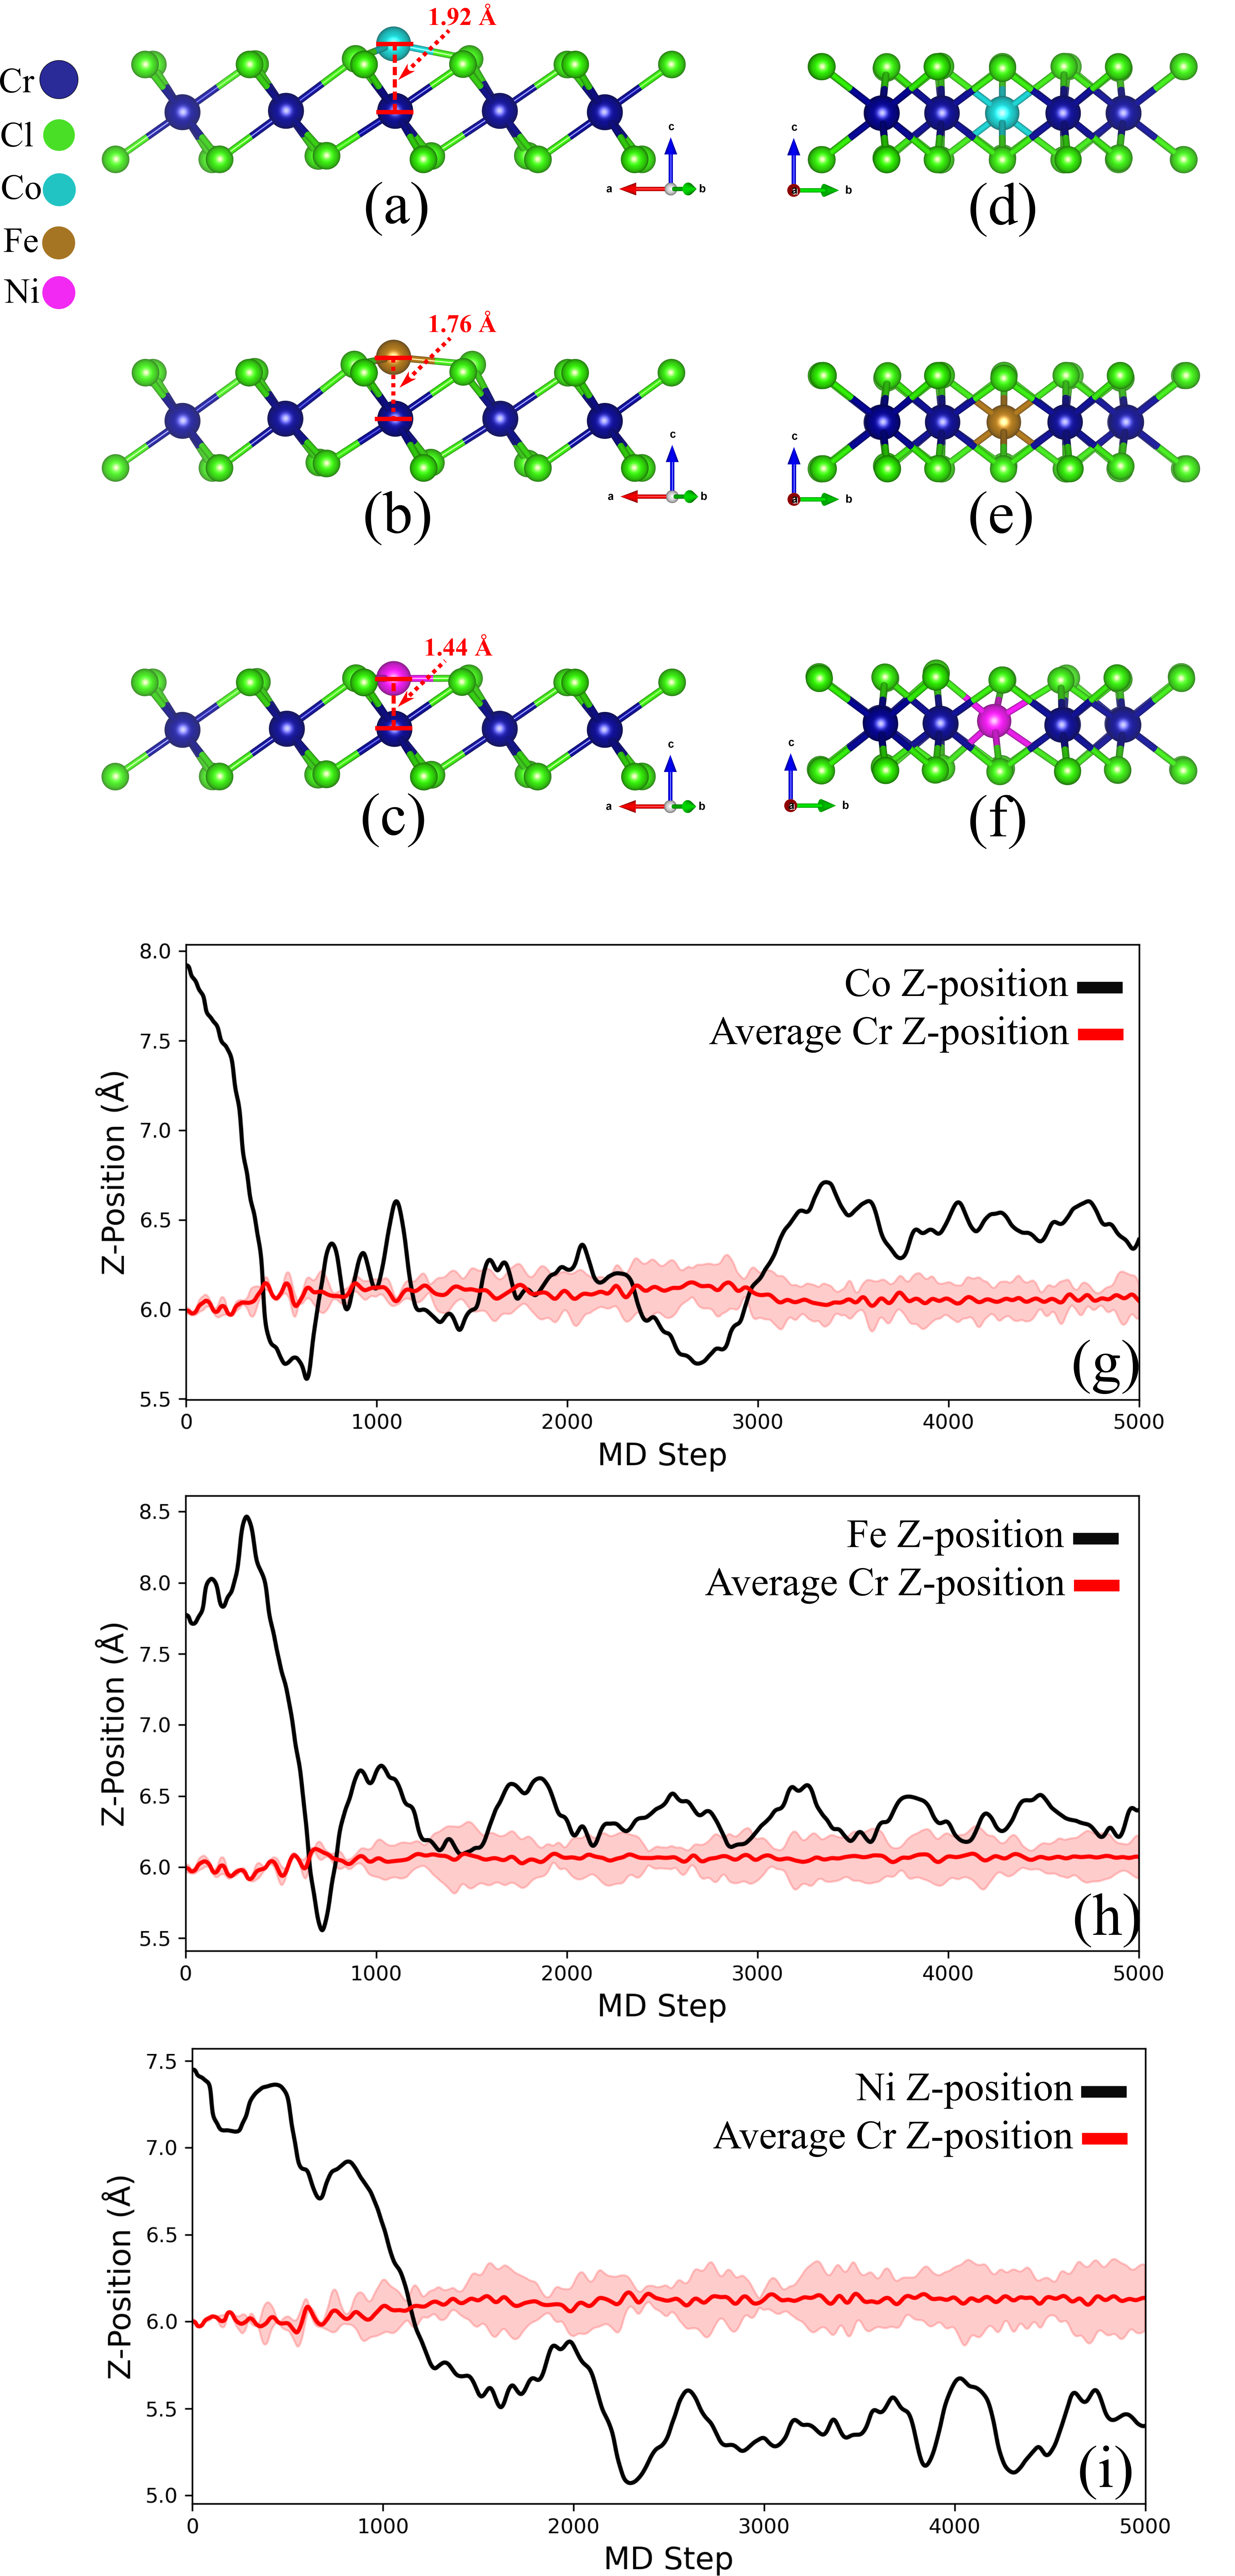
\includegraphics[width=0.98\linewidth]{figure/Fig_3.png}
    \caption{Structural and dynamical characterization of Co-, Fe-, and Ni-functionalized CrCl$_3$ monolayers. (a-c) Side views of the optimized Co-, Fe-, and Ni-adsorbed configurations at the hollow site of pristine CrCl$_3$, respectively, with the corresponding equilibrium adatom-surface distances. (d-f) Top views of the relaxed embedded configurations, in which Co, Fe, and Ni are incorporated into the hollow site of the CrCl$_3$ monolayer, respectively. (g-i) Time evolution of the vertical position ($z$ coordinate) of the adsorbed Co, Fe, and Ni atoms, respectively, obtained from \textit{ab initio} molecular dynamics (AIMD) simulations at 300 K. In each AIMD panel, the black curve denotes the instantaneous $z$ position of the adatom, whereas the red curve represents the average $z$ position of the Cr atoms in the CrCl$_3$ sheet. The figure compares the relaxed adsorption and embedding geometries and evaluates the thermal stability of the adsorbed transition-metal atoms relative to the Cr plane of the CrCl$_{3}$ monolayer.}
    \label{fig:Fig3}
\end{figure}

Figure~\ref{fig:Fig4} shows that both adsorption and embedding of Co, Fe, and Ni strongly perturb the semiconducting electronic structure of pristine CrCl$_3$. In all cases, impurity-derived states appear within or near the original band gap, and the PDOS indicates that these features arise mainly from the transition-metal $3d$ orbitals hybridized with Cr-$3d$ and Cl-$3p$ states. This behavior is consistent with the mixed Cr-$3d$/Cl-$3p$ character of the low-energy electronic structure of CrCl$_3$ reported previously \cite{Besbes2019,Soriano2020,Nharangatt2022}.

\begin{figure}[pos=H]
    \centering
    
\includegraphics[width=1.0\linewidth]{figure/Fig4.png}
    \caption{Electronic band structures and projected density of states (PDOS) of CrCl$_3$ functionalized with transition-metal atoms. (a), (c), and (e) show the band structures of the Co-, Fe-, and Ni-adsorbed CrCl$_3$ systems, respectively, while (b), (d), and (f) display the corresponding PDOS. Likewise, (g), (i), and (k) present the band structures of the Co-, Fe-, and Ni-embedded CrCl$_3$ configurations, respectively, whereas (h), (j), and (l) show their corresponding PDOS. The Fermi level is set to 0 eV in all panels. The PDOS highlights the contributions from Cr-$3d$, Cl-$3p$, and transition-metal $d$ orbitals, allowing a direct comparison between the adsorbed and embedded cases.}
    \label{fig:Fig4}
\end{figure}

For the adsorbed configurations [Fig.~\ref{fig:Fig4}(a-f)], Co and Fe introduce relatively localized states near the Fermi level while preserving the overall band profile of the host. In contrast, Ni adsorption produces a more pronounced reconstruction, with several Ni-$3d$-derived states appearing close to the Fermi level, consistent with its shorter equilibrium distance and stronger binding to the CrCl$_3$ surface. The embedded configurations [Fig.~\ref{fig:Fig4}(g-l)] lead to an even larger spectral reconstruction, with impurity states more clearly pinned inside the pristine gap, particularly for embedded Ni. These results indicate that transition-metal functionalization drives CrCl$_3$ toward a more electronically active state, which is expected to favor stronger interaction with adsorbed H \cite{Norskov_2005,Liao2022,pu2020single}. However, as discussed below, a stronger perturbation of the host electronic structure does not necessarily translate into the most favorable HER thermodynamics.

\begin{figure*}[h!]
    \centering
    
\includegraphics[width=0.85\linewidth]{figure/Fig5.png}
    \caption{Final relaxed geometries and energetic analysis of H adsorption on transition-metal-functionalized CrCl$_3$ monolayers. (a-c) Top and side views of the fully relaxed Co-, Fe-, and Ni-adsorbed CrCl$_3$ systems, respectively, after adsorption of a single H atom. (e-g) Top and side views of the optimized Co-, Fe-, and Ni-embedded CrCl$_3$ configurations, respectively, also in the presence of an adsorbed H atom. The indicated bond lengths highlight the local interaction between H, the transition-metal atom, and the local atomic environment of the CrCl$_3$ monolayer. (d) Interaction energy ($E_{\mathrm{int}}$), deformation energy ($E_{\mathrm{def}}$), adsorption energy ($E_{\mathrm{ads}}$), and adsorption free energy ($G_{\mathrm{ads}}$) for Co, Fe, and Ni adatoms adsorbed at the hollow site of CrCl$_3$. (h) The corresponding energetic contributions for Co, Fe, and Ni atoms embedded in the hollow site of the CrCl$_3$ monolayer.}
    \label{fig:Fig5}
\end{figure*}

Figure~\ref{fig:Fig5} shows that H adsorption is strongly dependent on the transition metal and on whether the metal is adsorbed or embedded in the CrCl$_3$ monolayer. For the adsorbed systems [Fig.~\ref{fig:Fig5}(a-c)], the H atom remains bound near the transition-metal center, with TM-H distances of 1.44, 1.57, and 1.46~\AA\ for Co, Fe, and Ni, respectively. The corresponding adsorption free energies are $G_{\mathrm{ads}} = 0.20$, 0.51, and 0.88~eV, showing that Co adsorption provides the most favorable H-binding thermodynamics, whereas Fe yields only a moderate improvement and Ni remains relatively less active. In contrast, the embedded configurations [Fig.~\ref{fig:Fig5}(e-g)] exhibit much larger adsorption free energies of 1.75, 1.36, and 3.62~eV for Co, Fe, and Ni, respectively, indicating that embedding the transition metals suppresses their activity for HER.



The energetic decomposition in Fig.~\ref{fig:Fig5}(d,h) clarifies the origin of this trend. For the adsorbed systems, Co shows the best balance between interaction and deformation terms, leading to an almost thermo-neutral adsorption energy, whereas Fe is penalized by a larger deformation cost and Ni by a weaker interaction term. The embedded cases exhibit a weaker response because all of them show positive interaction energies and, in the case of Ni, a particularly large deformation penalty. These results indicate that stronger metal--substrate coupling does not necessarily lead to better HER performance. Although Ni interacts most strongly with pristine CrCl$_3$, the most favorable catalytic response is obtained for adsorbed Co, where the local environment provides the best compromise between surface activation and H-binding thermodynamics. This behavior is consistent with the known sensitivity of CrCl$_3$ to chemical functionalization and further supports adsorbed Co/CrCl$_3$ as the most promising configuration among the systems considered here \cite{Luo2020,Wang2019,Gao2018,Mastrippolito2021,Mastrippolito2022,Zala2024}.

\section{Conclusions}

In summary, spin-polarized DFT calculations were used to investigate the effect of Co, Fe, and Ni incorporation on the structural, electronic, and catalytic properties of monolayer CrCl$_3$, considering both adsorbed and embedded configurations at the hollow site. The HER activity of pristine CrCl$_3$ was established as a baseline reference, showing that its stable 2D framework requires chemical activation to improve the H-binding thermodynamics. Transition-metal functionalization strongly modifies the CrCl$_3$ host, but the catalytic response is highly selective and depends on the local coordination of the metal center.

Among the systems examined, the Co-adsorbed configuration exhibits the most favorable HER behavior, providing the lowest H adsorption free energy and the best balance between surface activation and structural distortion. Fe adsorption yields only a moderate improvement, whereas Ni, despite its stronger interaction with the substrate, does not deliver the most favorable H-binding thermodynamics. In contrast, the embedded configurations show higher free energy barriers, highlighting that surface exposure of the active transition-metal sites is essential for achieving a favorable HER response. These results identify adsorbed Co/CrCl$_3$ as the most promising motif for HER and show that optimal catalytic activity in functionalized CrCl$_3$ is governed by the interplay between metal-substrate coupling, local structure, and H adsorption thermodynamics. Furthermore, although beyond the scope of the present study, investigating the interplay between intrinsic defects (such as vacancies) and transition-metal functionalization stands as a promising avenue for future work, particularly due to the potential to further tailor the local magnetic moments and enhance the catalytic response.


\section*{CRediT authorship contribution statement}
\begin{sloppypar}
    \textbf{Juan Rafael Gomez Quispe}: Conceptualization, Methodology, Software, Investigation, Writing - original draft. \textbf{Carlos Raul Primo Sapillado}: Investigation, Software, Validation. \textbf{Caique C. Oliveira}: Investigation, Software. \textbf{Chachi Rojas-Ayala}: Validation, Writing - review \& editing. \textbf{Pedro Alves da Silva Autreto}: Supervision, Project administration, Funding acquisition, Writing - review \& editing.
\end{sloppypar}

%\section*{Declaration of generative AI and AI-assisted technologies in the scientific writing process}
%During the preparation of this work the authors used Antigravity (a coding assistant based on Gemini) in order to assist with LaTeX formatting, bibliography management, and manuscript adaptation for journal submission. After using this tool, the authors reviewed and edited the content as needed and take full responsibility for the content of the publication.

\section*{Declaration of competing interest}
The authors declare that they have no known competing financial interests or personal relationships that could have appeared to influence the work reported in this paper.

\section*{Acknowledgment}

C. C. O. acknowledges the Sao Paulo Research Fundation (FAPESP process number 2024/11376-6). P. A. S. A. acknowledges Coordenacao de Aperfeicoamento de Pessoal de Nivel Superior (CAPES finance code 001), CNPq (grant 308428/2022-6) and National Institute of Science and Technology on Materials Informatics (grant no. 371610/2023-0). C. C. O., J. G. Q. and P. A. S. A. also acknowledge the UFABC Computation Multiuser Center (CCM) for the computational resources provided.

\section*{Data availability}
Data will be made available on request.

\bibliographystyle{elsarticle-num}

\bibliography{references}

\end{document}
